%=====================================================================
%  CSC111 -- Introduction to Computer Science
%  Unit 1: What is Computer Science?
%  University of Eswatini | Mr. J. S. Dlamini
%
%  BUILD NOTES
%  -----------
%  * Lecture build (overlays on):   pdflatex CSC111_Unit1.tex  (x2)
%  * Handout build (overlays off):  add "handout" to the class options
%  * Speaker notes on 2nd screen:   uncomment the \setbeameroption line
%  * Compile TWICE so the footer progress bar and page totals settle.
%=====================================================================

\documentclass[aspectratio=169]{beamer}
% \documentclass[aspectratio=169,handout]{beamer}   % <- printable handout

%---------------------------------------------------------------------
% Theme
%---------------------------------------------------------------------
\usetheme{Madrid}
\usecolortheme{beaver}
\setbeamertemplate{navigation symbols}{}

%---------------------------------------------------------------------
% Packages
%---------------------------------------------------------------------
\usepackage[utf8]{inputenc}
\usepackage[T1]{fontenc}          % FIX: was missing; needed for proper glyphs
\usepackage{lmodern}
\usepackage{graphicx}
\usepackage{amssymb}              % FIX: \checkmark lives here
\usepackage{booktabs}
\usepackage{tikz}
\usetikzlibrary{arrows.meta,positioning,shapes.geometric,fit,backgrounds}
\usepackage{fontawesome5}
\usepackage{xcolor}
\usepackage{pgfpages}
\usepackage{hyperref}

% Optional: QR codes for live polls. Uncomment if the package is installed.
% \usepackage{qrcode}

% Speaker notes on a second screen (presenter view). Uncomment to use.
% \setbeameroption{show notes on second screen=right}

%---------------------------------------------------------------------
% Colours
%---------------------------------------------------------------------
\definecolor{myNewColorA}{RGB}{206,8,20}      % UNESWA red
\definecolor{myNewColorB}{RGB}{26,168,217}    % Blue
\definecolor{myNewColorC}{RGB}{245,233,85}    % Yellow
\definecolor{darkblue}{RGB}{0,51,102}
\definecolor{lightblue}{RGB}{173,216,230}
\definecolor{softgrey}{RGB}{240,240,240}

% NOTE ON CONTRAST: yellow behind default text is hard to read on a bright
% projector. Foreground is forced to black below. If the front row still
% squints, swap myNewColorC for a deeper amber, e.g. RGB{230,190,40}.
\setbeamercolor*{palette primary}{bg=myNewColorC, fg=black}
\setbeamercolor*{palette secondary}{bg=myNewColorB, fg=white}
\setbeamercolor*{palette tertiary}{bg=myNewColorA, fg=white}
\setbeamercolor*{titlelike}{fg=myNewColorA}
\setbeamercolor*{title}{bg=myNewColorA, fg=white}
\setbeamercolor*{item}{fg=myNewColorA}
\setbeamercolor*{caption name}{fg=myNewColorA}
\usefonttheme{professionalfonts}

\hypersetup{colorlinks=true, linkcolor=myNewColorA, urlcolor=myNewColorB}

%---------------------------------------------------------------------
% Fonts
%---------------------------------------------------------------------
\setbeamerfont{title}{size=\large}
\setbeamerfont{subtitle}{size=\small}
\setbeamerfont{author}{size=\small}
\setbeamerfont{date}{size=\small}
\setbeamerfont{institute}{size=\small}

%---------------------------------------------------------------------
% Helper: image that degrades gracefully if the file is missing.
% Lets the deck compile on any machine even without the images/ folder.
%---------------------------------------------------------------------
\newcommand{\safeimage}[2][width=\textwidth]{%
  \IfFileExists{#2}%
    {\includegraphics[#1]{#2}}%
    {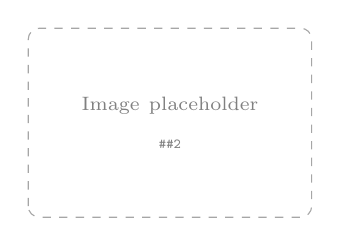
\begin{tikzpicture}
       \draw[dashed, rounded corners, gray!70] (0,0) rectangle (3.6,2.4);
       \node[gray, align=center, text width=3.2cm] at (1.8,1.2)
         {\scriptsize Image placeholder\\[2pt]\tiny\texttt{\detokenize{#2}}};
     \end{tikzpicture}}%
}

%---------------------------------------------------------------------
% Reusable "checkpoint" banner for the interactive frames
%---------------------------------------------------------------------
\newcommand{\checkpoint}[1]{%
  \begin{beamercolorbox}[sep=4pt, rounded=true, wd=\textwidth]{palette secondary}
    \centering\small\textbf{\faHandPaper\; CHECKPOINT --- #1}
  \end{beamercolorbox}%
}

%---------------------------------------------------------------------
% Footline with a thin progress bar
% (If this ever misbehaves on your TeX installation, comment the whole
%  block out -- everything else works without it.)
%---------------------------------------------------------------------
\setbeamertemplate{footline}{%
  \leavevmode%
  \hbox{%
    \begin{beamercolorbox}[wd=.30\paperwidth,ht=2.4ex,dp=1ex,center]{author in head/foot}%
      \usebeamerfont{author in head/foot}\insertshortauthor
    \end{beamercolorbox}%
    \begin{beamercolorbox}[wd=.50\paperwidth,ht=2.4ex,dp=1ex,center]{title in head/foot}%
      \usebeamerfont{title in head/foot}\insertshorttitle
    \end{beamercolorbox}%
    \begin{beamercolorbox}[wd=.20\paperwidth,ht=2.4ex,dp=1ex,center]{date in head/foot}%
      \usebeamerfont{date in head/foot}%
      \insertframenumber\,/\,\inserttotalframenumber
    \end{beamercolorbox}%
  }%
  \pgfmathsetmacro{\progressfrac}{\insertframenumber/\inserttotalframenumber}%
  \hbox to \paperwidth{%
    \color{myNewColorA}\rule{\progressfrac\paperwidth}{2.2pt}\hfil}%
  \vskip0pt%
}

%---------------------------------------------------------------------
% Title information
%---------------------------------------------------------------------
\titlegraphic{\safeimage[height=1.5cm]{UNESWA_logo.png}}
\title[CSC111 -- Unit 1]{Introduction to Computer Science}
\subtitle{CSC111 \textbar\ Unit 1: What is Computer Science?}
\author[J.\,S.\ Dlamini]{Mr.\ Johnson Dlamini}
\institute[jsdlamini@uniswa.sz]{Department of Computer Science\\The University of Eswatini}
\date{\today}          % FIX: bare \date was swallowing the next token

%---------------------------------------------------------------------
% Section divider: shows the whole map with the current section marked,
% so students always know where they are.
%---------------------------------------------------------------------
\AtBeginSection[]{
  \begin{frame}[plain]{Where we are}
    \tableofcontents[currentsection, hideallsubsections,
                     sectionstyle=show/shaded]
  \end{frame}
}

%=====================================================================
\begin{document}
%=====================================================================

\frame{\titlepage}

%---------------------------------------------------------------------
% HOOK -- open with a question, not an outline.
%---------------------------------------------------------------------
\begin{frame}{Before you sat down this morning\ldots}
  \begin{center}
    \Large Somebody had to \textbf{design} every system you already used today.
  \end{center}
  \vspace{0.4cm}
  \begin{columns}[T]
    \begin{column}{0.5\textwidth}
      \onslide<2->{%
      \begin{block}{Name them (30 seconds, out loud)}
        \small
        \begin{itemize}
          \item The alarm on your phone
          \item MoMo / e-Mali transfer for a kombi fare
          \item WhatsApp delivering a message across the country
          \item The system that registered you for this course
        \end{itemize}
      \end{block}}
    \end{column}
    \begin{column}{0.5\textwidth}
      \onslide<3->{%
      \begin{alertblock}{The question for this unit}
        Who builds those things, what do they actually \emph{know},
        and how is that different from simply \emph{using} a computer well?
      \end{alertblock}}
    \end{column}
  \end{columns}
\end{frame}
\note{Do not skip this. Let 3--4 students shout out answers before advancing.
      The whole unit lands better once they have supplied their own examples.
      Target: 3 minutes maximum.}

\begin{frame}{Outline}
  \tableofcontents
\end{frame}

%=====================================================================
\section{Course Overview}
%=====================================================================

\begin{frame}{CSC111 Module Overview}
  \begin{columns}[T]
    \begin{column}{0.6\textwidth}
      \textbf{What you'll learn:}
      \begin{itemize}[<+->]
        \item Definition of Computer Science
        \item History of computer science
        \item Qualities of a good computer scientist
        \item Related computing disciplines
        \item Overview of computers
        \item Algorithms, pseudo-code, and flowcharts
        \item Python programming fundamentals
      \end{itemize}
    \end{column}
    \begin{column}{0.4\textwidth}
      \centering
      \safeimage{images/ch1/computer_programming.png}\\[4pt]
      \small\textit{Programming and algorithms}
    \end{column}
  \end{columns}
\end{frame}
\note{Flag early: the last two bullets are where most of the assessment sits.}

\begin{frame}{Course Topics Coverage}
  \begin{columns}[T]
    \begin{column}{0.5\textwidth}
      \textbf{Core Topics:}
      \begin{itemize}
        \item Hardware \& Software
        \item Computer Generations
        \item Operating Systems
        \item Number Systems
        \item Database Management
        \item File Structure \& Handling
      \end{itemize}
    \end{column}
    \begin{column}{0.5\textwidth}
      \textbf{Advanced Topics:}
      \begin{itemize}
        \item Data Storage Hierarchy
        \item FOSS \& HFOSS
        \item Internet Applications
        \item Programming Languages
        \item Error Detection \& Correction
        \item Social \& Ethical Issues
      \end{itemize}
    \end{column}
  \end{columns}
  \vspace{0.4cm}
  \begin{alertblock}{Course Goal}
    By the end of this course you will have a solid grasp of computer science
    fundamentals \emph{and} you will be able to write working Python programs.
  \end{alertblock}
\end{frame}

%---------------------------------------------------------------------
% CHECKPOINT 1
%---------------------------------------------------------------------
\begin{frame}{Which of these is \emph{not} computer science?}
  \checkpoint{vote with your fingers, 1--4}
  \vspace{0.3cm}
  \begin{columns}[T]
    \begin{column}{0.55\textwidth}
      \begin{enumerate}
        \item Proving that no comparison sort can beat $n\log n$
        \item Designing the fraud checks for a mobile money service
        \item Re-installing Windows on the lab machines
        \item Training a model to map Eswatini's croplands from satellite images
      \end{enumerate}
    \end{column}
    \begin{column}{0.45\textwidth}
      \onslide<2->{%
      \begin{block}{Now}
        \small Hold up 1--4 fingers. Then take 30 seconds to defend your
        choice to the person next to you.
      \end{block}}
      \onslide<3->{%
      \begin{exampleblock}{Answer: (3)}
        \small Genuinely valuable IT work --- but it \emph{applies} an existing
        solution rather than designing a new one. Hold that distinction;
        we return to it at the end of this unit.
      \end{exampleblock}}
    \end{column}
  \end{columns}
\end{frame}
\note{Expect a big split between (3) and (4). That split IS the lesson --
      many students think "computer science = fixing computers".}

%=====================================================================
\section{Introduction to Computer Science}
%=====================================================================

\begin{frame}{What is Computer Science?}
  \begin{definition}
    Computer Science is the study of computers and computational systems ---
    what can be computed, how efficiently, and how to build systems that do it.
  \end{definition}
  \vspace{0.2cm}
  \begin{columns}[T]
    \begin{column}{0.55\textwidth}
      \textbf{Focus Areas:}
      \begin{itemize}[<+->]
        \item Software and software systems
        \item Theory, design, development
        \item Application of computing solutions
      \end{itemize}
    \end{column}
    \begin{column}{0.45\textwidth}
      \centering
      \safeimage[width=0.85\textwidth]{images/ch1/cs_overview.png}
    \end{column}
  \end{columns}
  \vspace{0.2cm}
  \onslide<4->{%
  \begin{block}{Key Distinction}
    Unlike electrical engineers, computer scientists focus primarily on
    \textbf{software} and on the \textbf{ideas} behind computation, rather than
    on the physical hardware.
  \end{block}}
\end{frame}

\begin{frame}{Principal Areas of Computer Science}
  \begin{columns}[T]
    \begin{column}{0.5\textwidth}
      \begin{itemize}[<+->]
        \item \faRobot\, Artificial Intelligence
        \item \faNetworkWired\, Computer Systems \& Networks
        \item \faShieldAlt\, Security          % FIX: \faShield does not exist
        \item \faDatabase\, Database Systems
        \item \faUser\, Human--Computer Interaction
      \end{itemize}
    \end{column}
    \begin{column}{0.5\textwidth}
      \begin{itemize}[<+->]
        \item \faEye\, Vision \& Graphics
        \item \faCalculator\, Numerical Analysis
        \item \faCode\, Programming Languages
        \item \faCogs\, Software Engineering
        \item \faDna\, Bioinformatics
      \end{itemize}
    \end{column}
  \end{columns}
  \vspace{0.4cm}
  \onslide<11->{%
  \begin{exampleblock}{Beyond Programming}
    Programming is the tool. Computer Science is algorithm design,
    performance analysis, and solving problems nobody has solved yet.
  \end{exampleblock}}
\end{frame}
\note{Ask: which of these ten did you not know existed? Usually bioinformatics
      and numerical analysis. Thirty seconds on each is enough.}

\begin{frame}{Computer Science Problem Spectrum}
  \begin{center}
    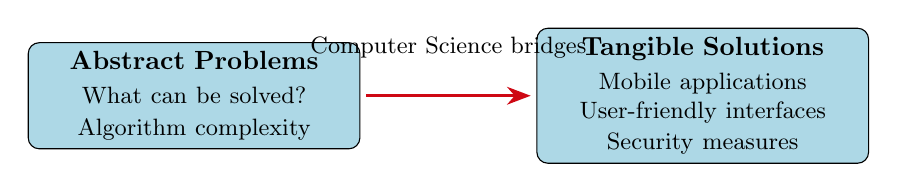
\begin{tikzpicture}[scale=0.95, transform shape]
      \node<1->[draw, rounded corners, fill=lightblue, text width=4.2cm,
                align=center] (abs) at (-3.4,0)
        {\textbf{Abstract Problems}\\[2pt]
         \small What can be solved?\\ Algorithm complexity};

      \node<2->[draw, rounded corners, fill=lightblue, text width=4.2cm,
                align=center] (tan) at (3.4,0)
        {\textbf{Tangible Solutions}\\[2pt]
         \small Mobile applications\\ User-friendly interfaces\\ Security measures};

      \draw<3->[-{Stealth[length=3mm]}, very thick, myNewColorA]
        (-1.1,0) -- (1.1,0);
      \node<3->[above=8pt, font=\small] at (0,0.1) {Computer Science bridges};
    \end{tikzpicture}
  \end{center}
  \vspace{0.3cm}
  \onslide<4->{%
  \begin{alertblock}{CS Professional Range}
    Computer scientists work across the whole span --- from theoretical
    foundations to the app on your phone.
  \end{alertblock}}
\end{frame}

%---------------------------------------------------------------------
% MYTH vs REALITY -- addresses what is actually in their heads right now
%---------------------------------------------------------------------
\begin{frame}{Myth vs.\ Reality}
  \begin{columns}[T]
    \begin{column}{0.5\textwidth}
      \begin{beamercolorbox}[sep=4pt,rounded=true]{palette tertiary}
        \centering\textbf{The Myth}
      \end{beamercolorbox}
      \vspace{4pt}
      \begin{itemize}[<+->]
        \item ``Computer science is just coding.''
        \item ``You must be a maths genius.''
        \item ``AI will make this degree worthless.''
        \item ``You need an expensive laptop to start.''
      \end{itemize}
    \end{column}
    \begin{column}{0.5\textwidth}
      \begin{beamercolorbox}[sep=4pt,rounded=true]{palette secondary}
        \centering\textbf{The Reality}
      \end{beamercolorbox}
      \vspace{4pt}
      \begin{itemize}[<+->]
        \item Coding is one skill among design, analysis and communication.
        \item You need persistence with logic. Maths gets \emph{built}, not inherited.
        \item AI raises the value of people who understand what it is doing.
        \item Everything in this course runs on free, open-source tools.
      \end{itemize}
    \end{column}
  \end{columns}
\end{frame}
\note{This slide buys you attention for the rest of the semester. Be honest
      about the AI one -- students have heard the scare stories.}

%=====================================================================
\section{Computer Scientists}
%=====================================================================

\begin{frame}{Who is a Computer Scientist?}
  \begin{definition}
    A computer scientist has acquired knowledge of Computer Science --- the
    theoretical foundations of information and computation, together with their
    practical application.
  \end{definition}
  \vspace{0.3cm}
  \begin{columns}[T]
    \begin{column}{0.6\textwidth}
      \textbf{Computer scientists:}
      \begin{itemize}[<+->]
        \item Design computers and software
        \item Develop information technologies
        \item Apply computing principles to new domains
        \item Are distinguished by theoretical expertise
        \item Focus on innovation and complex problems
      \end{itemize}
    \end{column}
    \begin{column}{0.4\textwidth}
      \centering
      \safeimage[width=0.8\textwidth]{images/ch1/computer_scientist.png}
    \end{column}
  \end{columns}
\end{frame}

\begin{frame}{Qualities of a Good Computer Scientist}
  \begin{columns}[T]
    \begin{column}{0.5\textwidth}
      \textbf{Technical Foundation:}
      \begin{itemize}[<+->]
        \item Strong mathematical background
        \item Algorithm design expertise
        \item Problem-solving skills
        \item Innovation mindset
        \item Technology application
      \end{itemize}
    \end{column}
    \begin{column}{0.5\textwidth}
      \textbf{Soft Skills:}
      \begin{itemize}[<+->]
        \item Logical thinking
        \item Good communication
        \item Attention to detail
        \item Team collaboration
      \end{itemize}
    \end{column}
  \end{columns}
  \vspace{0.6cm}
  \onslide<10->{%
  \begin{exampleblock}{Innovation Areas}
    \small Robotics, Computer Vision, Intelligent Systems, Bioinformatics
  \end{exampleblock}}
\end{frame}
\note{Ask which column students think employers complain about most.
      Answer: the right-hand one, every time.}

\begin{frame}{Computer Scientist Responsibilities}
  \begin{block}{Core Activities}
    \begin{itemize}
      \item Think of new ways to use computers
      \item Explore innovative applications
      \item Develop solutions for complex computing problems
      \item Supervise programming teams
      \item Develop encryption and data protection schemes
      \item Lead large software development projects
    \end{itemize}
  \end{block}
  \begin{columns}[T]
    \begin{column}{0.5\textwidth}
      \textbf{Career Progression:}
      \begin{itemize}
        \item Industry: management and technical lead roles
        \item Academia: researchers, lecturers, professors
        \item Independent consulting
        \item Entrepreneurship
      \end{itemize}
    \end{column}
    \begin{column}{0.5\textwidth}
      \begin{alertblock}{Continuous Learning}
        Technology moves fast. The degree teaches you how to keep learning ---
        that is the durable part.
      \end{alertblock}
    \end{column}
  \end{columns}
\end{frame}

%---------------------------------------------------------------------
% CHECKPOINT 2 -- think / pair / share
%---------------------------------------------------------------------
\begin{frame}{Rank them}
  \checkpoint{think --- pair --- share, 3 minutes}
  \vspace{0.3cm}
  \begin{center}
    \large Of the nine qualities we just listed, which \textbf{three} matter
    most in a first job?
  \end{center}
  \vspace{0.4cm}
  \begin{columns}[T]
    \begin{column}{0.32\textwidth}
      \begin{block}{1. Think (60s)}
        \small Write your top three down. Alone, no talking.
      \end{block}
    \end{column}
    \begin{column}{0.32\textwidth}
      \onslide<2->{\begin{block}{2. Pair (90s)}
        \small Compare with your neighbour. Agree on one combined top three.
      \end{block}}
    \end{column}
    \begin{column}{0.32\textwidth}
      \onslide<3->{\begin{block}{3. Share (30s)}
        \small Two pairs report back. We tally on the board.
      \end{block}}
    \end{column}
  \end{columns}
  \vspace{0.3cm}
  \onslide<4->{\centering
    \hyperlink{ans:qualities}{\beamerbutton{What employers actually say}}}
\end{frame}

\begin{frame}{What employers actually say}
  \hypertarget{ans:qualities}{}
  \begin{exampleblock}{The pattern}
    Across surveys of graduate hiring in the region, the complaints are rarely
    about algorithms. They are about \textbf{communication}, \textbf{attention
    to detail}, and \textbf{working in a team}.
  \end{exampleblock}
  \vspace{0.3cm}
  \begin{block}{Why this matters for you}
    \begin{itemize}
      \item Technical skill gets you the interview.
      \item The other column gets you the job --- and the promotion.
      \item Group work in this course is practice, not filler.
    \end{itemize}
  \end{block}
  % TODO: cite a specific regional employer survey here before delivery.
\end{frame}

%=====================================================================
\section{Why Study Computer Science?}
%=====================================================================

\begin{frame}{Reasons to Study Computer Science}
  \begin{enumerate}[<+->]
    \item \textbf{The digital age needs computer scientists}
      \begin{itemize}
        \item Software now sits inside almost every service you touch
        \item Someone has to design, secure and maintain it
      \end{itemize}
      \vspace{0.2cm}
    \item \textbf{The skills travel}
      \begin{itemize}
        \item The same problem-solving applies to banking, health, agriculture
        \item Remote work makes the market larger than any one country
      \end{itemize}
      \vspace{0.2cm}
    \item \textbf{Needed in every industry}
      \begin{itemize}
        \item Universal application across all sectors
        \item Problem-solving in science, engineering and healthcare
      \end{itemize}
  \end{enumerate}
\end{frame}
\note{The original "big salaries" claim was removed -- unsourced, and it sets
      up disappointment. The next slide makes the concrete case instead.}

\begin{frame}{Where the work actually is}
  \begin{columns}[T]
    \begin{column}{0.5\textwidth}
      \textbf{In Eswatini and the region:}
      \begin{itemize}[<+->]
        \item Telecommunications operators
        \item Banking and mobile money platforms
        \item Government digital services and revenue systems
        \item Health information systems
        \item Agriculture and geospatial services
        \item Research and higher education
      \end{itemize}
    \end{column}
    \begin{column}{0.5\textwidth}
      \onslide<7->{%
      \begin{block}{And beyond}
        \begin{itemize}
          \item Remote contracts for firms abroad
          \item Open-source contribution as a public portfolio
          \item Your own product --- the barrier to entry is a laptop
        \end{itemize}
      \end{block}}
      \onslide<8->{%
      \begin{alertblock}{Be realistic}
        Demand is real, but it rewards demonstrated work.
        Start building things in first year, not final year.
      \end{alertblock}}
    \end{column}
  \end{columns}
\end{frame}

\begin{frame}{Digital Age Impact}
  \begin{center}
    \safeimage[width=0.28\textwidth]{images/ch1/digital_age.png}
  \end{center}
  \vspace{0.2cm}
  \begin{columns}[T]
    \begin{column}{0.5\textwidth}
      \textbf{Everywhere computing:}
      \begin{itemize}
        \item Mobile applications
        \item Web services
        \item IoT devices
        \item Cloud computing
      \end{itemize}
    \end{column}
    \begin{column}{0.5\textwidth}
      \textbf{The CS role:}
      \begin{itemize}
        \item Design software solutions
        \item Ensure system reliability
        \item Optimise performance
        \item Enhance user experience
      \end{itemize}
    \end{column}
  \end{columns}
\end{frame}

%=====================================================================
\section{History and Related Disciplines}
%=====================================================================

%---------------------------------------------------------------------
% FIX: the original used a "timeline" environment that does not exist
%      in any loaded package -- this frame would not compile.
%      Replaced with a staged TikZ timeline.
%---------------------------------------------------------------------
\begin{frame}{Evolution of Computer Science}
  \begin{center}
    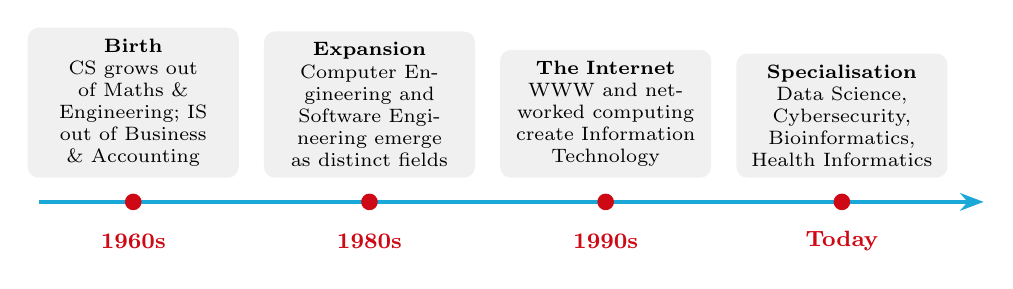
\begin{tikzpicture}[x=1.5cm, every node/.style={align=center}]
      % the spine
      \draw[-{Stealth[length=3mm]}, very thick, myNewColorB] (0.2,0) -- (8.2,0);

      % tick marks and decade labels
      \foreach \x/\yr in {1/1960s, 3/1980s, 5/1990s, 7/Today}{
        \fill[myNewColorA] (\x,0) circle (3pt);
        \node[font=\footnotesize\bfseries, text=myNewColorA] at (\x,-0.5) {\yr};
      }

      \node<2->[anchor=south, text width=2.4cm, font=\scriptsize,
                fill=softgrey, rounded corners, inner sep=4pt] at (1,0.3)
        {\textbf{Birth}\\ CS grows out of Maths \& Engineering;
         IS out of Business \& Accounting};

      \node<3->[anchor=south, text width=2.4cm, font=\scriptsize,
                fill=softgrey, rounded corners, inner sep=4pt] at (3,0.3)
        {\textbf{Expansion}\\ Computer Engineering and Software Engineering
         emerge as distinct fields};

      \node<4->[anchor=south, text width=2.4cm, font=\scriptsize,
                fill=softgrey, rounded corners, inner sep=4pt] at (5,0.3)
        {\textbf{The Internet}\\ WWW and networked computing create
         Information Technology};

      \node<5->[anchor=south, text width=2.4cm, font=\scriptsize,
                fill=softgrey, rounded corners, inner sep=4pt] at (7,0.3)
        {\textbf{Specialisation}\\ Data Science, Cybersecurity,
         Bioinformatics, Health Informatics};
    \end{tikzpicture}
  \end{center}
  \vspace{0.2cm}
  \onslide<6->{%
  \begin{exampleblock}{The pattern}
    \small Every wave splits off a new discipline. The one you will graduate
    into probably does not have a name yet.
  \end{exampleblock}}
\end{frame}
\note{If time allows, put faces to it: Lovelace, Turing, Hopper -- and ask when
      computing first arrived at UNESWA. Students engage with stories, not decades.}

\begin{frame}{Modern Computing Disciplines (1990s--Present)}
  \begin{block}{Software Engineering Growth}
    Driven by the need for rigorous development methods for:
    \begin{columns}[T]
      \begin{column}{0.5\textwidth}
        \begin{itemize}
          \item Military command systems
          \item Avionics and aerospace
        \end{itemize}
      \end{column}
      \begin{column}{0.5\textwidth}
        \begin{itemize}
          \item Operating systems
          \item Complex computer games
        \end{itemize}
      \end{column}
    \end{columns}
  \end{block}
  \begin{block}{Information Technology Emergence}
    \begin{itemize}
      \item Explosive growth of the Internet and WWW in the 1990s
      \item Rapid expansion of networked computing
      \item A new discipline focused on practical IT application
    \end{itemize}
  \end{block}
  \begin{exampleblock}{Emerging Fields}
    \small Informatics, Health Informatics, Business Informatics, Data Science,
    Bioinformatics, Cybersecurity, Digital Forensics
  \end{exampleblock}
\end{frame}

\begin{frame}{ACM Computing Disciplines}
  \textbf{The five core disciplines recognised by the ACM:}
  \vspace{0.2cm}
  \begin{description}[<+->]
    \item[\faMemory\, Computer Engineering (CE)]
      Design and construction of computers and computer-based systems.
      Hardware, software and communications.
    \item[\faLaptopCode\, Computer Science (CS)]
      Theoretical foundations through to cutting-edge development.
      The broadest foundation.
    \item[\faBuilding\, Information Systems (IS)]
      Integrating IT solutions with business processes to meet
      organisational needs.
    \item[\faServer\, Information Technology (IT)]
      Meeting user needs through selection, deployment and administration
      of computing technology.
    \item[\faCogs\, Software Engineering (SE)]
      Building reliable, efficient and affordable software systems using
      engineering principles.
  \end{description}
\end{frame}

\begin{frame}{Discipline Comparison}
  \begin{center}
    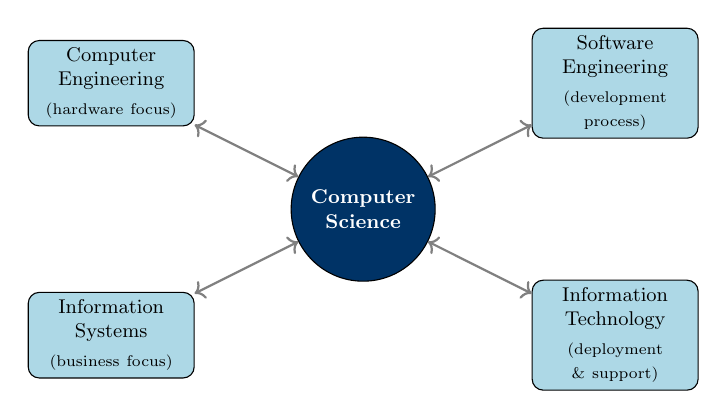
\begin{tikzpicture}[scale=0.8, transform shape,
                        disc/.style={rectangle, draw, rounded corners,
                                     fill=lightblue, text width=2.4cm,
                                     align=center, font=\small}]
      \node<1->[circle, draw, fill=darkblue, text=white, text width=1.9cm,
                align=center, font=\small\bfseries] (cs) at (0,0)
        {Computer Science};

      \node<2->[disc] (ce) at (-4,2)  {Computer Engineering\\[2pt]\scriptsize(hardware focus)};
      \node<3->[disc] (se) at (4,2)   {Software Engineering\\[2pt]\scriptsize(development process)};
      \node<4->[disc] (is) at (-4,-2) {Information Systems\\[2pt]\scriptsize(business focus)};
      \node<5->[disc] (it) at (4,-2)  {Information Technology\\[2pt]\scriptsize(deployment \& support)};

      \draw<2->[<->, thick, gray] (cs) -- (ce);
      \draw<3->[<->, thick, gray] (cs) -- (se);
      \draw<4->[<->, thick, gray] (cs) -- (is);
      \draw<5->[<->, thick, gray] (cs) -- (it);
    \end{tikzpicture}
  \end{center}
  \onslide<6->{%
  \begin{alertblock}{The CS advantage}
    Computer Science gives the most comprehensive foundation --- which is what
    lets graduates move between all four of the surrounding fields.
  \end{alertblock}}
\end{frame}

%---------------------------------------------------------------------
% CHECKPOINT 3 -- scenario matching
%---------------------------------------------------------------------
\begin{frame}{Match the job to the discipline}
  \checkpoint{shout it out}
  \vspace{0.3cm}
  \small
  \begin{enumerate}[<+->]
    \item A bank needs its new loan process mapped onto its existing software.
          \onslide<6->{\hfill\textbf{\color{myNewColorA}IS}}
    \item A hospital's patient records system keeps crashing under load; someone
          must redesign how it is built and tested.
          \onslide<7->{\hfill\textbf{\color{myNewColorA}SE}}
    \item A farm wants a low-power sensor board designed to read soil moisture.
          \onslide<8->{\hfill\textbf{\color{myNewColorA}CE}}
    \item The campus needs its network, servers and user accounts kept running.
          \onslide<9->{\hfill\textbf{\color{myNewColorA}IT}}
    \item Nobody knows whether a fair, efficient algorithm for allocating those
          hospital beds even exists.
          \onslide<10->{\hfill\textbf{\color{myNewColorA}CS}}
  \end{enumerate}
  \vspace{0.3cm}
  \onslide<11->{%
  \begin{exampleblock}{Notice}
    \small Only the last one asks whether a solution is \emph{possible}.
    That question is the heart of computer science.
  \end{exampleblock}}
\end{frame}
\note{Reveal each answer only after the room has committed. If they answer
      instantly, push back: "why not SE?"}

%=====================================================================
\section{Computer Literacy and Competency}
%=====================================================================

\begin{frame}{Computer Literacy}
  \begin{definition}
    Computer literacy is understanding what a computer is and how it can be
    used as a resource.
  \end{definition}
  \vspace{0.4cm}
  \textbf{Key components:}
  \begin{itemize}[<+->]
    \item Understanding computer fundamentals
    \item Knowledge of software types
    \item Awareness of different computer systems
    \item Basic operational skills
    \item Information literacy
  \end{itemize}
  \vspace{0.3cm}
  \onslide<6->{%
  \begin{alertblock}{Employment impact}
    Across the labour market, applicants without basic computing skills are
    shut out of a large and growing share of advertised positions.
    % TODO: replace with a cited figure (e.g. an ILO or national labour survey)
    %       before delivery. The original "80\%" claim had no source.
  \end{alertblock}}
\end{frame}

\begin{frame}{Computer Competency}
  \begin{definition}
    Computer competency means applying your computing skills to meet real
    information needs and improve productivity.
  \end{definition}
  \vspace{0.3cm}
  \textbf{Competency features:}
  \begin{itemize}
    \item Transfer basic skills to unfamiliar systems
    \item Adapt to different software environments
    \item Solve problems using computing tools
    \item Enhance personal and professional productivity
  \end{itemize}
  \vspace{0.4cm}
  \begin{columns}[T]
    \begin{column}{0.5\textwidth}
      \textbf{Professional benefits:}
      \begin{itemize}
        \item Career advancement
        \item Problem-solving efficiency
        \item Adaptability to new tools
      \end{itemize}
    \end{column}
    \begin{column}{0.5\textwidth}
      \textbf{Personal benefits:}
      \begin{itemize}
        \item Enhanced learning
        \item Increased productivity
        \item Creativity and entertainment
      \end{itemize}
    \end{column}
  \end{columns}
\end{frame}
\note{One-liner that lands: literacy is knowing Word. Competency is sitting
      down at software you have never seen and being useful within an hour.}

\begin{frame}{Information Literacy}
  \begin{block}{Beyond computer skills}
    Information literacy enables you to:
    \begin{itemize}[<+->]
      \item \textbf{Find} relevant information efficiently
      \item \textbf{Analyse} information critically
      \item \textbf{Use} information effectively in your career
      \item \textbf{Evaluate} source credibility
      \item \textbf{Synthesise} information from multiple sources
    \end{itemize}
  \end{block}
  \vspace{0.2cm}
  \onslide<6->{%
  \begin{exampleblock}{Why it is urgent now}
    \small Search engines and AI assistants will hand you a confident answer
    whether or not it is correct. Evaluating the source is now part of the job.
  \end{exampleblock}}
\end{frame}

%=====================================================================
\section{Professionals vs Users}
%=====================================================================

\begin{frame}{Computer Professionals}
  \begin{definition}
    A computer professional understands the technical aspects of computing
    systems and builds or maintains them.
  \end{definition}
  \vspace{0.3cm}
  \begin{description}[<+->]
    \item[\faCode\, Software Engineer / Programmer]
      Design, write, test, implement and maintain software.
    \item[\faProjectDiagram\, Systems Analyst]
      Analyse, design and develop entire information systems for organisations.
    \item[\faNetworkWired\, Network Administrator]
      Manage, maintain and update network infrastructure.
    \item[\faDatabase\, Database Administrator]
      Design and coordinate database activity: access privileges, security,
      backup, recovery and performance.
  \end{description}
\end{frame}

\begin{frame}{Computer Users (End-Users)}
  \begin{definition}
    A computer user is a person without extensive technical knowledge who uses
    computers for work or personal tasks.
  \end{definition}
  \vspace{0.4cm}
  \begin{columns}[T]
    \begin{column}{0.5\textwidth}
      \textbf{Characteristics:}
      \begin{itemize}
        \item Limited technical knowledge
        \item Focus on application use
        \item Task-oriented approach
        \item Learning-focused mindset
        \item Productivity goals
      \end{itemize}
    \end{column}
    \begin{column}{0.5\textwidth}
      \textbf{Examples:}
      \begin{itemize}
        \item Computer operators
        \item Data entry operators
        \item Accountants
        \item Administrative clerks
        \item General office workers
      \end{itemize}
    \end{column}
  \end{columns}
  \vspace{0.3cm}
  \begin{exampleblock}{Growth potential}
    This is not a permanent category. With interest and practice, users become
    experts --- and experts become professionals.
  \end{exampleblock}
\end{frame}

\begin{frame}{Professional vs.\ User}
  \small
  \begin{center}
    \begin{tabular}{@{}p{2.6cm}p{4.6cm}p{4.6cm}@{}}
      \toprule
      \textbf{Aspect} & \textbf{Computer Professional} & \textbf{Computer User}\\
      \midrule
      Knowledge level   & Deep technical understanding   & Basic operational knowledge\\
      \addlinespace
      Primary focus     & System design and development  & Application usage\\
      \addlinespace
      Problem solving   & Creates technical solutions    & Uses existing solutions\\
      \addlinespace
      Career path       & Specialised technical roles    & Various non-technical roles\\
      \addlinespace
      Learning approach & Continuous technical education & Task-specific learning\\
      \bottomrule
    \end{tabular}
  \end{center}
  \vspace{0.4cm}
  \begin{alertblock}{Important}
    Not every computer professional is a computer scientist. Computer science
    adds theoretical depth and the ability to produce new knowledge.
  \end{alertblock}
\end{frame}

%---------------------------------------------------------------------
% CHECKPOINT 4 -- callback to the opening question
%---------------------------------------------------------------------
\begin{frame}{Back to slide 3}
  \checkpoint{closing argument, 2 minutes}
  \vspace{0.4cm}
  \begin{center}
    \Large ``All computer professionals cannot be referred to as
    computer scientists.''
  \end{center}
  \vspace{0.5cm}
  \begin{columns}
    \begin{column}{0.5\textwidth}
      \onslide<2->{\begin{block}{Left half of the room}
        Argue \textbf{for} the statement.
      \end{block}}
    \end{column}
    \begin{column}{0.5\textwidth}
      \onslide<2->{\begin{block}{Right half of the room}
        Argue \textbf{against} it.
      \end{block}}
    \end{column}
  \end{columns}
  \vspace{0.4cm}
  \onslide<3->{\centering\small
    One sentence each. The strongest sentence wins the point.}
\end{frame}
\note{Time-box this hard at 2 minutes. It is a warm-up for the written
      assignment, not the assignment itself.}

%=====================================================================
\section{Summary and Next Steps}
%=====================================================================

\begin{frame}{Unit Summary}
  \textbf{Key learning outcomes achieved:}
  \vspace{0.3cm}
  \begin{columns}[T]
    \begin{column}{0.5\textwidth}
      \begin{itemize}
        \item[\checkmark] Defined Computer Science
        \item[\checkmark] Explored CS history and evolution
        \item[\checkmark] Identified related computing disciplines
        \item[\checkmark] Understood reasons to study CS
      \end{itemize}
    \end{column}
    \begin{column}{0.5\textwidth}
      \begin{itemize}
        \item[\checkmark] Learned the qualities of good computer scientists
        \item[\checkmark] Distinguished literacy from competency
        \item[\checkmark] Compared professionals and users
        \item[\checkmark] Gained foundational CS knowledge
      \end{itemize}
    \end{column}
  \end{columns}
  \vspace{0.4cm}
  \begin{alertblock}{Next Steps}
    This foundation prepares you for programming concepts and Python,
    algorithms and data structures, computer systems and networks, and
    software development methodologies.
  \end{alertblock}
\end{frame}

\begin{frame}{Take-home work}
  \textbf{Written (submit before the next lecture):}
  \begin{enumerate}
    \item List four reasons why you would like to be a computer scientist.
    \item Explain three qualities of a good computer scientist.
    \item List and explain five related computing disciplines.
    \item Discuss: ``All computer professionals cannot be referred to as
          computer scientists.'' (One page maximum.)
  \end{enumerate}
  \vspace{0.3cm}
  \begin{block}{Group discussion topics (tutorial)}
    \begin{itemize}
      \item Compare the different computing disciplines
      \item Analyse career paths in computer science
      \item Evaluate the importance of computer literacy across professions
      \item Discuss ethical considerations in computer science
    \end{itemize}
  \end{block}
\end{frame}

\begin{frame}{Looking Forward}
  \vspace{0.5cm}
  \begin{center}
    {\Large\textbf{Welcome to Computer Science.}}\\[0.6cm]
    \begin{minipage}{0.75\textwidth}
      \centering\small
      You arrived today already using a dozen systems other people designed.
      By the end of this course you will have designed one yourself.
    \end{minipage}
  \end{center}
  \vspace{0.8cm}
  % Optional live poll / feedback QR code -- needs \usepackage{qrcode}
  % \begin{center}\qrcode[height=2.2cm]{https://your-feedback-url}\end{center}
  \begin{center}
    \textbf{Questions and Discussion}\\[0.2cm]
    \small\texttt{jsdlamini@uniswa.sz}
  \end{center}
\end{frame}

\end{document}